%%%%%%%%%%%%%%%%%%%%%%%%%%%%%%%%%%%%%%%%%
% Simple Sectioned Essay Template
% LaTeX Template
%
% This template has been downloaded from:
% http://www.latextemplates.com
%
% Note:
% The \lipsum[#] commands throughout this template generate dummy text
% to fill the template out. These commands should all be removed when 
% writing essay content.
%
%%%%%%%%%%%%%%%%%%%%%%%%%%%%%%%%%%%%%%%%%

%----------------------------------------------------------------------------------------
%	PACKAGES AND OTHER DOCUMENT CONFIGURATIONS
%----------------------------------------------------------------------------------------

\documentclass[12pt]{article} % Default font size is 12pt, it can be changed here

\usepackage{geometry} % Required to change the page size to A4
\geometry{a4paper} % Set the page size to be A4 as opposed to the default US Letter

\usepackage{graphicx} % Required for including pictures

\usepackage{float} % Allows putting an [H] in \begin{figure} to specify the exact location of the figure
\usepackage{wrapfig} % Allows in-line images such as the example fish picture

\usepackage{lipsum} % Used for inserting dummy 'Lorem ipsum' text into the template
\usepackage{subfigure}

\linespread{1.2} % Line spacing

%\setlength\parindent{0pt} % Uncomment to remove all indentation from paragraphs

\graphicspath{{Pictures/}} % Specifies the directory where pictures are stored

\begin{document}

%----------------------------------------------------------------------------------------
%	TITLE PAGE
%----------------------------------------------------------------------------------------

\begin{titlepage}

\newcommand{\HRule}{\rule{\linewidth}{0.5mm}} % Defines a new command for the horizontal lines, change thickness here

\center % Center everything on the page

\textsc{\LARGE Universit\'a Tor Vergata}\\[1.5cm] % Name of your university/college
\textsc{\Large Corso di Laurea di Ingegneria Informatica}\\[0.5cm] % Major heading such as course name
\textsc{\large A.A. 2016-2017}\\[0.5cm] % Minor heading such as course title

\HRule \\[0.4cm]
{ \huge \bfseries Mobile Sniffing Tool}\\[0.4cm] % Title of your document
{ \bfseries Progetto di Sicurezza Informatica e Internet}\\[0,4cm]
\HRule \\[1.5cm]

\begin{minipage}{0.4\textwidth}
\begin{flushleft} \large
\emph{Autori:}\\
Paolo \textsc{Salom\'e}\\
Stefano \textsc{Agostini} % Your name
\end{flushleft}
\end{minipage}
~
\begin{minipage}{0.4\textwidth}
\begin{flushright} \large
\emph{Supervisori:}\\
Prof. Giuseppe \textsc{Italiano}\\ 
Dr. Marco \textsc{Querini}  % Supervisor's Name
\end{flushright}
\end{minipage}\\[8,5cm]

{\large \today}\\[3cm] % Date, change the \today to a set date if you want to be precise

%\includegraphics{Logo}\\[1cm] % Include a department/university logo - this will require the graphicx package

\vfill % Fill the rest of the page with whitespace

\end{titlepage}

%----------------------------------------------------------------------------------------
%	TABLE OF CONTENTS
%----------------------------------------------------------------------------------------

\tableofcontents % Include a table of contents

\newpage % Begins the essay on a new page instead of on the same page as the table of contents 

%----------------------------------------------------------------------------------------
%	INTRODUCTION
%----------------------------------------------------------------------------------------

\section{Introduzione} % Major section

Nella societ\'a odierna vi \'e un larga diffusione di applicazioni mobile di messagistica che espongono implicitamente gli utenti a problematiche riguardanti la privacy. Infatti fino a qualche mese fa i dati in transito di Whatsapp (e.g.) erano in chiaro e quindi accedibili facilmente da chiunque utilizzasse una qualsiasi applicazione per lo sniffing (e.g. Whireshark). Tuttavia attualmente molte delle applicazioni di messaggistica hanno rimediato interamente o parzialmente utilizzando tecniche di crittografia end-to-end. 
L'obiettivo del nostro progetto \'e la realizzazione di una applicazione per sistemi mobile Android che all'interno di una certa rete wifi catturi i dati in transito e li filtri in base ad un flag. In tal modo ci preponiamo l'obiettivo di isolare i pacchetti dati per ogni applicazione di messaggistica presa in considerazione e analizzarli.
 
%------------------------------------------------

%\subsection{Subsection 1} % Sub-section

%\lipsum[1] % Dummy text

%------------------------------------------------

%\subsection{Subsection 2} % Sub-section

%\lipsum[2] % Dummy text

%------------------------------------------------

%\subsubsection{Subsubsection 1} % Sub-sub-section

%\lipsum[3] % Dummy text

%\begin{figure}[H] % Example image
%\center{
\includegraphics[width=0.5\linewidth]{placeholder}}
%\caption{Example image.}
%\label{fig:speciation}
%\end{figure}

%------------------------------------------------

%\subsubsection{Subsubsection 2} % Sub-sub-section

%\lipsum[4] % Dummy text

%----------------------------------------------------------------------------------------
%	MAJOR SECTION 1
%----------------------------------------------------------------------------------------

\section{Descrizione dell'Applicazione} % Major section

Per realizzare uno \textit{sniffer Android} c'erano due strade alternative da poter seguire: sfruttare le \textit{Android VPN} oppure utilizzare l'eseguibile \textit{C tcpdump}. L'approccio \textit{Android VPN} consiste nella creazione di un'interfaccia \textit{VPNService}, gestita da una applicazione in \textit{userspace}, che una volta attivata forza tutto il traffico del \textit{device} ad attraversarla. Tuttavia questo approccio non permette la cattura di pacchetti appartenenti a dispositivi diversi da quello ospitante l'applicazione. Per utilizzare il secondo approccio \'e necessario che il dispositivo abbia i permessi di \textit{root} in quanto verr\'a eseguito uno \textit{script bash tcpdump}, il quale si occuper\'a di catturare i pacchetti. Inoltre questa libreria permette di sfruttare la scheda di rete in uso in varie modalit\'a (e.g. \textit{promiscous mode, monitor mode}) qualora il dispositivo lo consenta. La possibilit\'a di sfruttare a pieno le potenzialit\'a della scheda di rete ci ha indotto a scegliere \textit{tcpdump}.     

%------------------------------------------------

\subsection{Tcpdump} % Sub-section

Il comando \textit{bash} dell'eseguibile \textit{tcpdump} permette l'inserimento di alcuni parametri che permettono la visualizzazione dei pacchetti in vari formati. Nel caso della nostra applicazione utilizziamo i seguenti parametri:

\begin{itemize}
\item \textbf{-i} : seguito dal nome dell'interfaccia, per specificare dove porsi in ascolto (e.g. wlan0)
\item \textbf{-XX} in alternativa a \textbf{-A}: il primo stampa l'header di ogni pacchetto e i dati in esadecimale e \textit{ASCII} mentre il secondo non stampa l'esadecimale
\item \textbf{-tttt}: stampa la data corrente davanti l'header di ogni pacchetto in formato \textit{YYYY-MM-DD hh:mm:ss:dddddd}
\end{itemize}

Di seguito inseriamo un pacchetto di esempio stampato da bash come risultato del comando \textit{sudo tcpdump -i wlan0 -XX -tttt} (figure \ref{fig:XX}) e del comando \textit{sudo tcpdump -i wlan0 -A -tttt} (figure \ref{fig:A}).

\begin{figure}[H] % Example image
\center{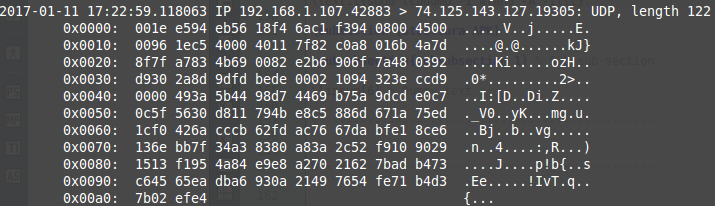
\includegraphics[scale=0.6]{tcpdump_XX.png}}
\caption{Con opzione -XX}\label{fig:XX}
\end{figure}

\begin{figure}[H] % Example image
\center{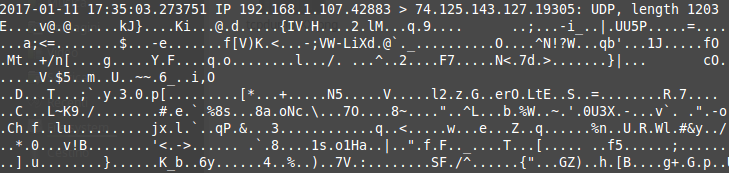
\includegraphics[scale=0.6]{tcpdump_A.png}}
\caption{Con opzione -A}\label{fig:A}
\end{figure}

\newpage
\subsection{Struttura APK}
La nostra \textit{APK} si compone di due \textit{Activity} e due \textit{Service}:

\begin{itemize}
\item L'\textit{Activity} di cattura espone un'interfaccia semplice per impostare la modalit\'a di cattura (specificare il \textit{flag} \textit{hex mode}). Successivamente l'utente pu\'o specificare il nome del file sul quale vuole che vengano salvati i pacchetti. Infine è possibile attivare il servizio di cattura.
\item L'\textit{Activity} di filtraggio si occupa di fornire all'utente un elenco dei file contenenti i pacchetti, salvati dall'applicazione stessa nelle precedenti catture. Selezionato il file da elenco è possibile inserire la parola chiave di ricerca. Mediante il servizio di filtraggio \'e vengono scanditi i pacchetti e visualizzati in una lista soltanto quelli contenenti la parola desiderata.
\item Il \textit{Service} di cattura si occupa dell'invocazione del comando \textit{tcpdump} con le opzioni e il nome del file passati dall'\textit{Activity} di cattura, redirezionando l'output su quest'ultimo. Quando questo servizio viene interrotto si esegue il comando bash \textit{pkill tcpdump} per terminare il comando dello \textit{sniffer}. 
\item Il \textit{Service} di filtraggio agisce sul file selezionato esaminando ogni pacchetto e inserendolo in una lista visualizzata a schermo solo se contiene la \textit{keyword} fornita, all'interno dell'\textit{header} o del \textit{body}.
\end{itemize}
 
Di seguito inseriamo degli \textit{screen} dell'applicazione appena descritta (figure \ref{fig:apk}).
 
 
\begin{figure}[htbp]
\centering%
\subfigure[Activity di cattura\label{fig:apk1}]%
{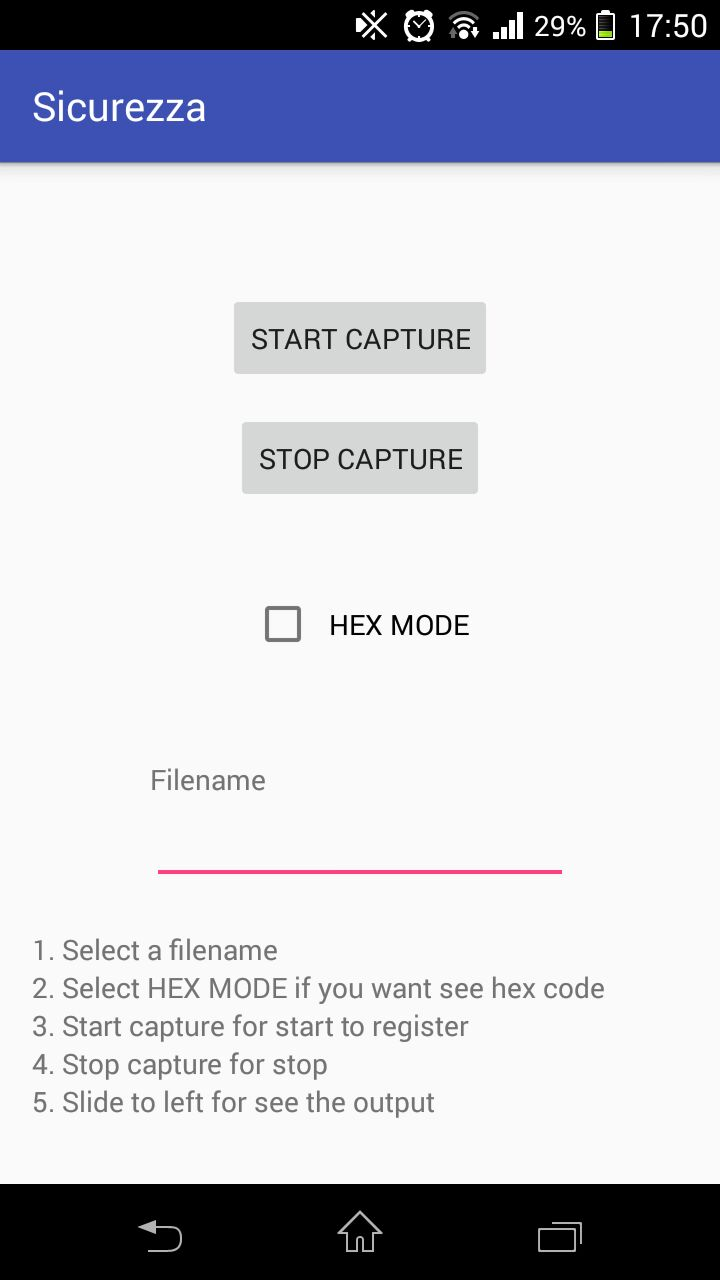
\includegraphics[scale=0.2]{./activity1.jpeg}}\qquad\qquad
\subfigure[Activity di filtraggio\label{fig:apk2}]%
{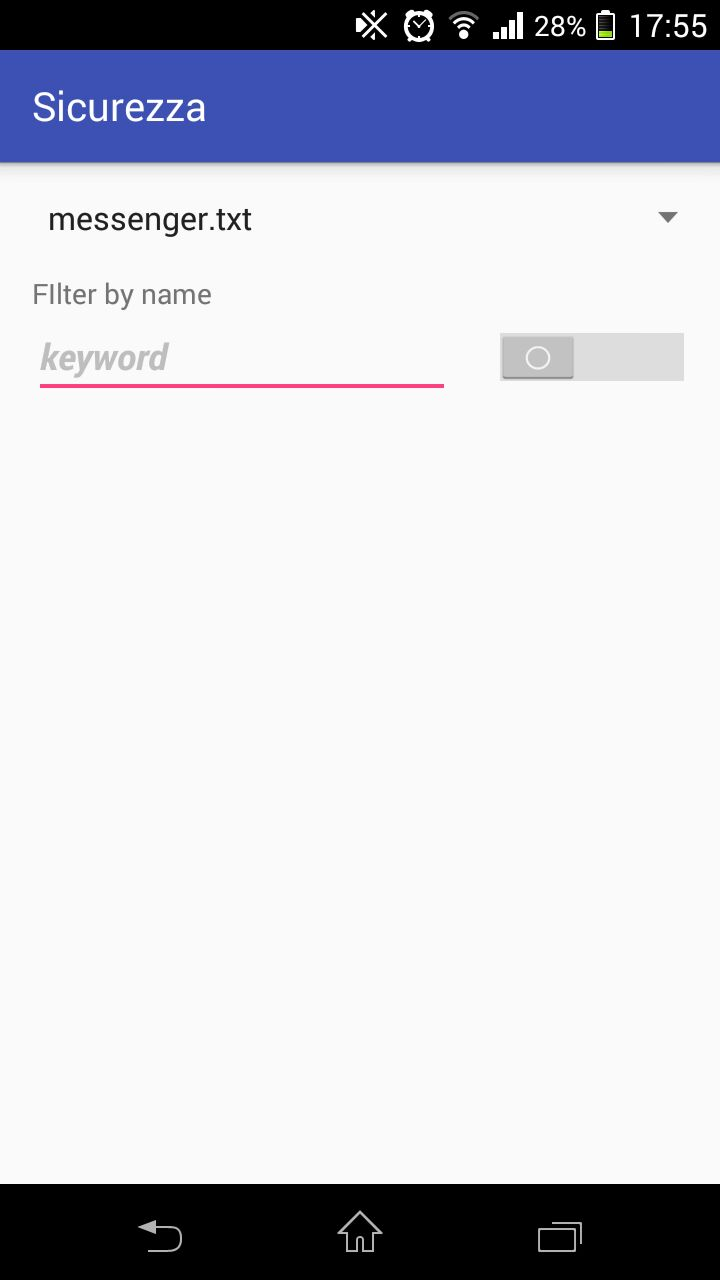
\includegraphics[scale=0.2]{./activity2.jpeg}}\qquad\qquad
\\
\subfigure[Lista di file\label{fig:filelist}]%
{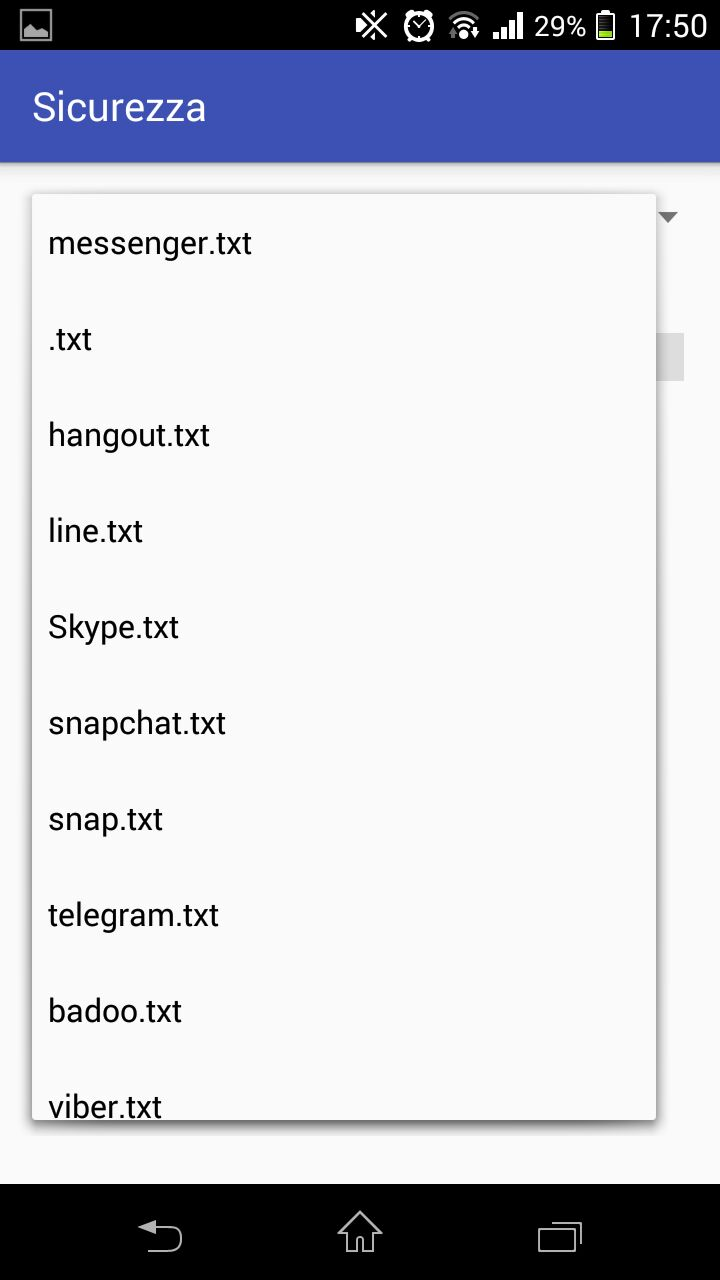
\includegraphics[scale=0.2]{./filelist.jpeg}}\qquad\qquad
\subfigure[Pacchetti filtrati\label{fig:apk2active}]%
{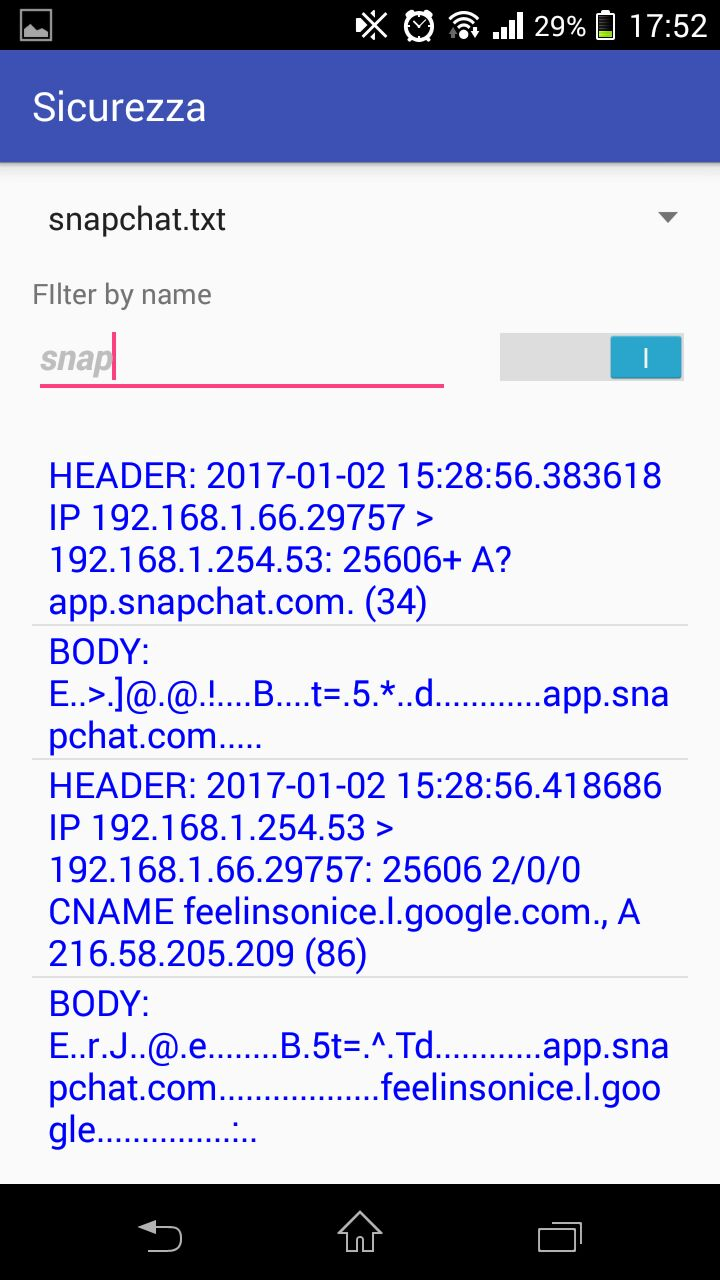
\includegraphics[scale=0.2]{./activity2active.jpeg}}
\caption{Pagine dell'applicazione\label{fig:apk}}
\end{figure} 
 
\subsubsection{Subsubsection 1} % Sub-sub-section

\lipsum[6] % Dummy text

%------------------------------------------------


%------------------------------------------------


%----------------------------------------------------------------------------------------
%	MAJOR SECTION X - TEMPLATE - UNCOMMENT AND FILL IN
%----------------------------------------------------------------------------------------

%\section{Content Section}

%\subsection{Subsection 1} % Sub-section

% Content

%------------------------------------------------

%\subsection{Subsection 2} % Sub-section

% Content

%----------------------------------------------------------------------------------------
%	CONCLUSION
%----------------------------------------------------------------------------------------

\section{Conclusion} % Major section

\lipsum[12-13]

%----------------------------------------------------------------------------------------
%	BIBLIOGRAPHY
%----------------------------------------------------------------------------------------

\begin{thebibliography}{99} % Bibliography - this is intentionally simple in this template

\bibitem[Figueredo and Wolf, 2009]{Figueredo:2009dg}
Figueredo, A.~J. and Wolf, P. S.~A. (2009).
\newblock Assortative pairing and life history strategy - a cross-cultural
  study.
\newblock {\em Human Nature}, 20:317--330.
 
\end{thebibliography}

%----------------------------------------------------------------------------------------

\end{document}